\documentclass{article}
\usepackage[a4paper, total={6in, 10in}]{geometry}

\title{MM20B059}
\author{Sumanth Hegde}
\date{July 2021}

\usepackage{natbib}
\usepackage{graphicx}

\begin{document}

\maketitle

\section{The Gamma Function Equation}
{\Large$$\Gamma(x)=\int_{0}^{\infty}e^{-t}t^{x-1}dt$$}
\subsection{Variables}
$\Gamma(x)$=The value of Gamma Function\newline
$x$=value at which Gamma Function is to be evaluated
\begin{figure}[h!]
\centering
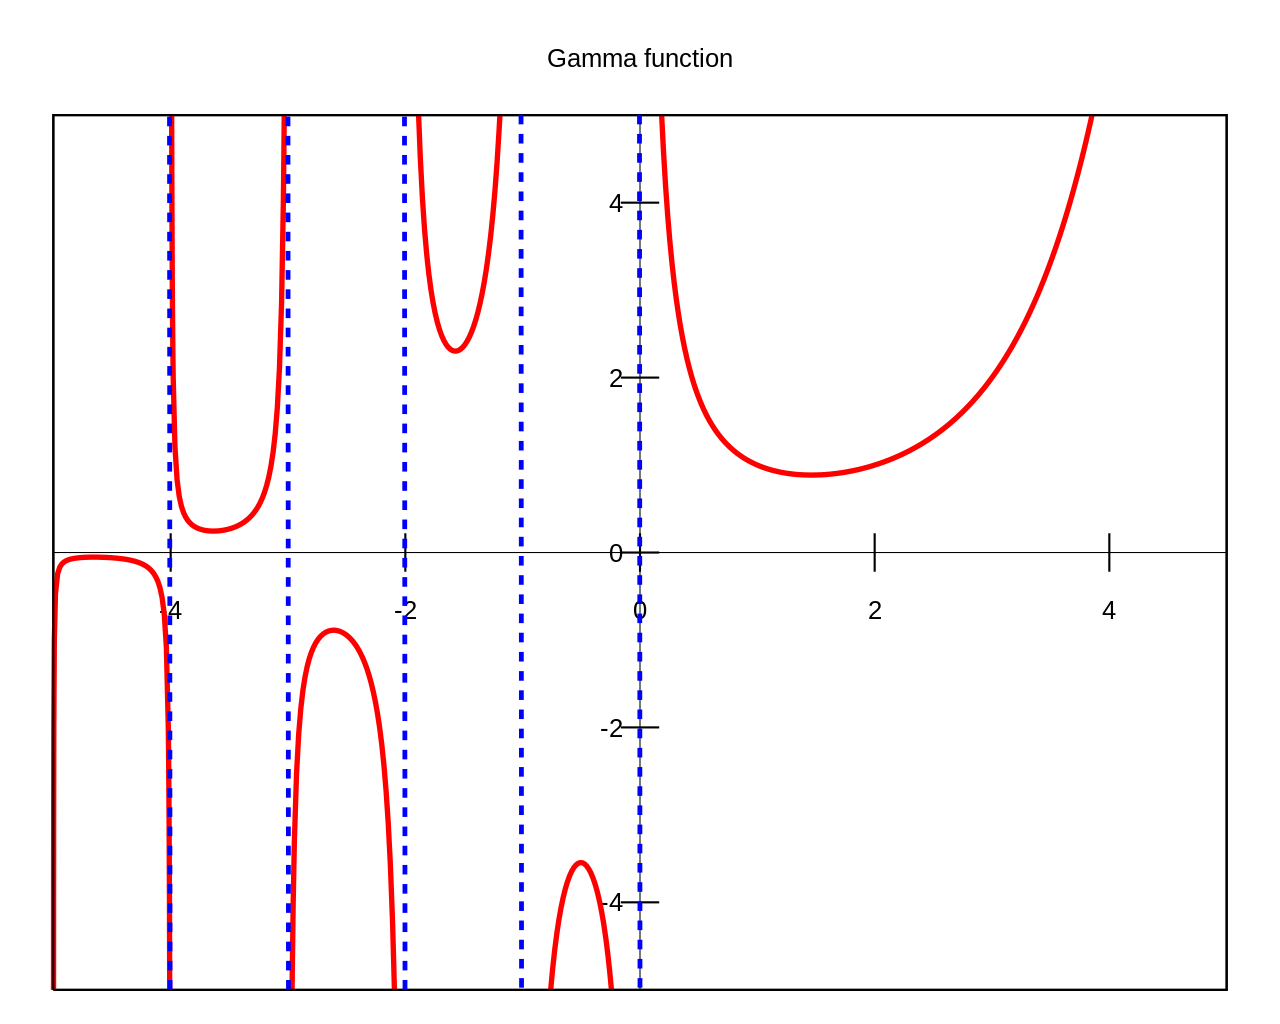
\includegraphics[scale=0.23]{gamma.png}
\caption{Gamma Function Plot}
\label{fig:gamma}
\end{figure}

\section{Description}
In mathematics, the gamma function (represented by $\Gamma$) is one commonly used extension of the factorial function to continuous and complex numbers. The gamma function is defined for all complex numbers except the non-positive integers as an improper integral as given in the equation above. For positive integers, $\Gamma(x)=(x-1)!$~\cite{enwiki:1029050612}

\bibliographystyle{plain}
\bibliography{references}

\end{document}
